\documentclass{standalone}
\usepackage{tikz}

\begin{document}

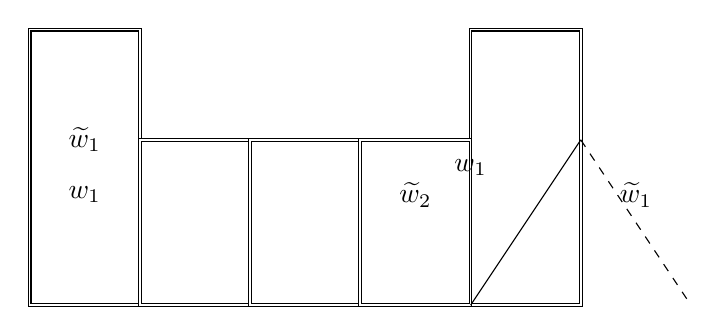
\begin{tikzpicture}[scale=0.7]
  % Draw the first layer with double lines
  \draw[double] (-4,0) rectangle (-2,5);
  \draw[double] (4,0) rectangle (6,5);

  % Draw the second layer with double lines
  \draw[double] (-2,0) rectangle (0,3);
  \draw[double] (0,0) rectangle (2,3);
  \draw[double] (2,0) rectangle (4,3);

  % Draw the third layer with single line
  \draw (4,0) -- (6,3);

  % Draw the fourth layer with dashed line
  \draw[dashed] (6,3) -- (8,0);

  % Add labels for the convolution operations
  \node at (-3,3) {$\widetilde{w}_1$};
  \node at (3,2) {$\widetilde{w}_2$};
  \node at (7,2) {$\widetilde{w}_1$};

  % Add labels for the skip connections
  \node at (-3,2) {\(w_1\)};
  \node at (4,2.5) {\(w_1\)};
\end{tikzpicture}

\end{document}